\documentclass[12pt]{report}
\usepackage[utf8]{inputenc}
\usepackage[T1]{fontenc}
\usepackage[english]{babel}
\usepackage{graphicx}
\usepackage{amsmath}
\usepackage{amssymb}
\usepackage{hyperref}
\usepackage{epsf}
\usepackage{float}
\usepackage{geometry}
\geometry{hmargin=3.5cm, vmargin=2.5cm}
\usepackage[squaren]{SIunits}
\usepackage{listings}
\usepackage{color}
\definecolor{mygreen}{RGB}{70, 180, 90}
\definecolor{mylilas}{RGB}{255, 117, 45}
\definecolor{cadr}{rgb}{0.89, 0.0, 0.13}
\graphicspath{{DWGs/}}
\usepackage{graphicx}
\usepackage{wrapfig}
\usepackage{graphicx}
\usepackage{multicol}
\usepackage{enumitem}
\usepackage{xcolor}
\usepackage{framed}
\definecolor{shadecolor}{RGB}{139, 231, 3}

\usepackage{tcolorbox}
\definecolor{mycolor}{rgb}{0.122, 0.435, 0.698}

\newtcbox{\mb}{nobeforeafter,colframe=mycolor,colback=mycolor!10!white,boxrule=0.5pt,arc=4pt,
  boxsep=0pt,left=6pt,right=6pt,top=3pt,bottom=3pt,tcbox raise base}


\begin{document}

\begin{titlepage}
    \begin{center}

		\vspace*{6cm}
        \LARGE     
		
        \Huge
        \textbf{My journey through learning Boundary Layers}
        
        \vspace*{1cm}
        


        \vspace{2cm}
        
        \LARGE
        K. Zdybal

        \vspace{6cm}
		\Large

		\vspace{1cm}

 		October, 2017
	\end{center}
\end{titlepage}


% EX_LIBRIS_PAGE_TEMPLATE START ===============================

\thispagestyle{empty}
\begin{center}
    
\vspace*{4cm}

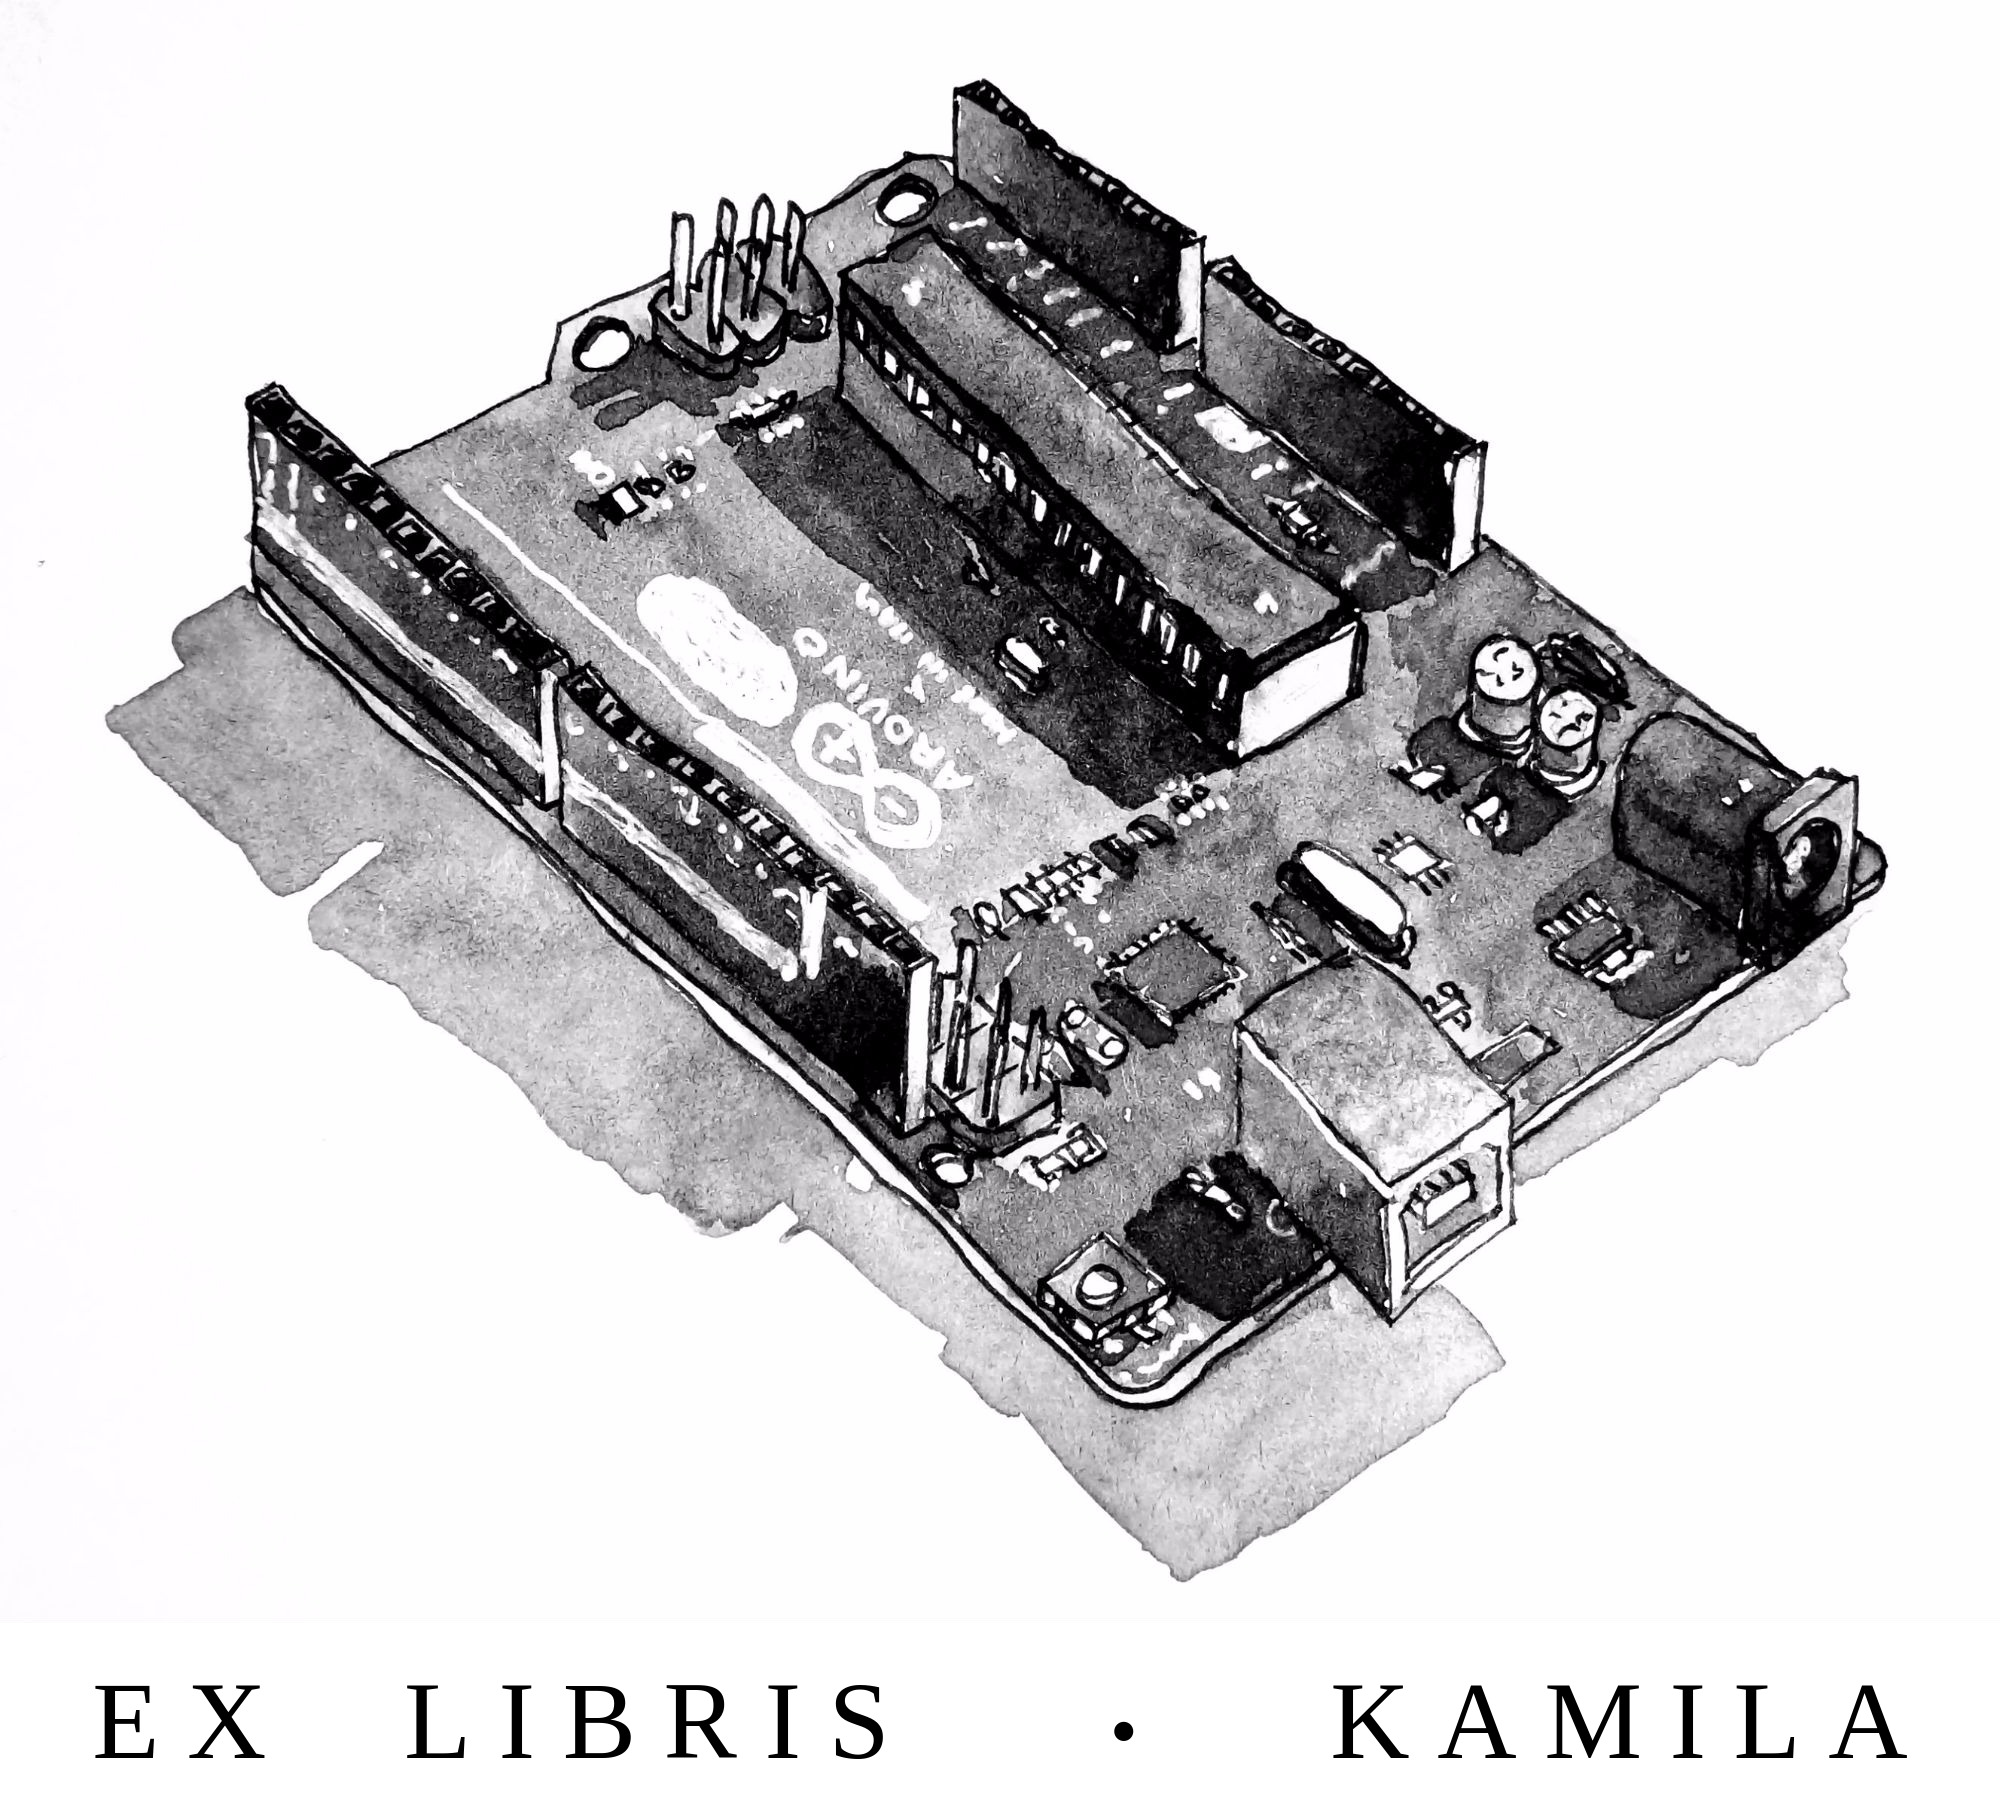
\includegraphics[width = 70mm]{arduino_dwg.jpg}

\vspace*{2cm}

Copyright \textcopyright \, Kamila Zdybał, 2017

For more documents similar to this one 

visit me on GitHub: @camillejr

To contact me personally drop me a line at:

\verb|kamilazdybal@gmail.com|

\end{center}
\newpage

% EX_LIBRIS_PAGE_TEMPLATE END ================================

\setlength{\parindent}{0cm}

\clearpage


\tableofcontents



\setlength{\parskip}{1em}
\renewcommand{\baselinestretch}{1.0}


\newpage


\chapter{Introduction} \label{chap:intro}

In October 2017 I have decided that I will be studying boundary layers for minimum 25 minutes every day.


\section{Mission objectives} \label{chap:objectives}

When you decide to sacrifice time and effort to pursue certain field of interest you'd better find very strong and realistic reasons for why you do that. Of course, it also has to bring you everyday pleasure but in the times when it stops being a pleasure (and those times will come), you have to have something more to motivate you. At those times, when you're tired and don't feel like studying and you know that your brain won't absorb enough knowledge and that reading a textbook will be a nightmare, there are your reasons why you wanted to do that in the first place. They are your babies screaming at night and you just have to get up and feed them.

These are my reasons for why I study boundary layers:

\begin{enumerate}

\item I want to gain maths knowledge used in fluid dynamics, so that next subjects will be of less struggle in understanding calculus and become really the struggle to understand fluid dynamics.

\item I want to understand Navier-Stokes equations. I want to gain intuitive feel for them and become comfortable about what every term means. I want to see their full power and see what their limitations are.

\item I want to build a knowledge toolbox to create Matlab / Python codes to simulate boundary layers phenomena.

\item I want to write this PDF that will contain a bunch of my-way-explanations of "difficult" concepts which will hopefully one day become a guide (that I always needed to find) for someone.

\item I want to become better at fluid dynamics in general so that even when there are amazing places like the Von Karman Institute which can't take me for their programs because the government of my country didn't support their research, there might still be people who would like to help. You know: "be so good that they can't ignore you".

\end{enumerate}



\section{How to make it interesting} \label{chap:interesting}

This is a list of things that bring the pleasure to my studies:



\begin{enumerate}

\item Imagining how what I've learned could be used.

\item Imagining experiments I could do to verify what was said in the book.

\item Making thought experiments, sometimes imagining "what-if-worlds" that do not exist.

\item Doing things my way and doing things new way. Finding new ways to make things more interesting.

\item Explaining things on a white board / card board as if I was presenting it to someone.

\item Preparing an illustrative drawing to explain what was said in the book.

\item Writing LaTeX documents.

\item Talking with friends.


\end{enumerate}



\section{The learning curve} \label{chap:learning_curve}




\section{The learning observations} \label{chap:learning_observations}



\chapter{Preliminaries}



\section{World without friction} \label{chap:without_friction}

Imagine the world without friction.

Now imagine, that you move the palms of your hand agains each other.

Do you feel the "shear" or "drag" on your hands?

- No. With no friction this is not present.

Do you feel the "pressing" of each palm on the other?

- Yes! I can feel it!

Perfect! There is no reason why you shouldn't. The forces perpendicular to your palms get transported from one to the other just fine.\footnote{Interesting distraction: can you think of a way to build a "frictionless world" simulator, one that will allow you to feel the push on your hands when they get in close contact but at the same time you will not experience the shear when sliding your hands?}

Now, the same thing happens when we make an assumption that the fluid is perfect, ergo frictionless. Any object that such fluid will flow around will not experience the shear stress (or the drag). It will however experience the pressure force perpendicular to its outline.

There is a big consequence that comes from the above "monologue": if you want to study the drag on a body immersed in a fluid, you have to look at the world of friction.

That's why it's the high time to leave the frictionless considerations. It's of not much use in the subject of boundary layers - or the science of what happens at the very edge between. Get ready for the ride in the world of friction.







\section{Understanding substantial derivative} \label{chap:deriv}

The substantial derivative is damn important. I've already had a chance to find about this in my previous pursuits of fluid mechanics. I remember it has been a challenge to really understand what the substantial derivative means and when I began my studying of BLs I realized that I either already forgot what I've once learned or I've never really understand it.

But this time I need to understand it deeply! So let's find a way to do that.

Imagine that you're walking on the streets of London with a bag of muffins. Every once in a while you reach to the bag to pick another muffin that you then endeavour because you're really a big fan of pastry and because the day is enjoyable and you want to feel happy.

On the street that you're currently strolling on there's a really good bakery and the croissants look so delicious from the shop window that you just have to walk inside to buy a few.

Then you take your bag of goodies and walk into the Buckingham Palace Gardens to eat the hell out of it. By the end of your walk you've finished the whole bag.

Now you take a seat on the park bench and in the warm sunlight you begin to wonder:

...if I were to analyse the change in time of the amount of pastry products inside my bag... what would it be...? Well, some change was due to me constantly eating the pastry through my whole journey. But there was also an increase in pastry when I bought the croissants. If I wasn't walking near that awesome bakery, there wouldn't be, so some change had to be dependent of where I was walking. Maybe if I chose my paths recklessly I might have even lost a few muffins to the outside world! Let me call the change of pastry in time by the term:

$\frac{Dp}{Dt}$

$p$ - standing for pastry

Then I'm going to call the continuous change due to eating (and independent of my path) the Local Change of $p$ ($LC_p$). And there has to be the term which is dependent of where I went which I'm going to call the Advective Change of $p$ ($AC_p$).

So the total change of pastry in time is simply the sum of the two:

$\frac{Dp}{Dt} = LC_p + AC_p$













\newpage

\begin{thebibliography}{50}



\end{thebibliography}

\end{document}
